\documentclass[a4paper,11pt]{article}
\usepackage[left=2cm,right=2cm,
top=2cm,bottom=2cm,bindingoffset=0cm]{geometry}

%%% Работа с русским языком
\usepackage{cmap}					% поиск в PDF
\usepackage{mathtext} 				% русские буквы в формулах
\usepackage[T2A]{fontenc}			% кодировка
\usepackage[utf8]{inputenc}			% кодировка исходного текста
\usepackage[english,russian]{babel}	% локализация и переносы

%%% Дополнительная работа с математикой
\usepackage{amsmath,amsfonts,amssymb,amsthm,mathtools} % AMS
\usepackage{icomma} % "Умная" запятая: $0,2$ --- число, $0, 2$ --- перечисление

%% Номера формул
%\mathtoolsset{showonlyrefs=true} % Показывать номера только у тех формул, на которые есть \eqref{} в тексте.
%\usepackage{leqno} % Нумерация формул слева

%% Свои команды
%\DeclareMathOperator{\sgn}{\mathop{sgn}}

%% Перенос знаков в формулах (по Львовскому)
%\newcommand*{\hm}[1]{#1\nobreak\discretionary{}
	%	{\hbox{$\mathsurround=0pt #1$}}{}}

%%% Работа с картинками
\usepackage{graphicx}  % Для вставки рисунков
\graphicspath{{images/}{images2/}}  % папки с картинками
\setlength\fboxsep{6pt} % Отступ рамки \fbox{} от рисунка
\setlength\fboxrule{1pt} % Толщина линий рамки \fbox{}
\usepackage{wrapfig} % Обтекание рисунков текстом

%%% Работа с таблицами
%\usepackage{array,tabularx,tabulary,booktabs} % Дополнительная работа с таблицами
%\usepackage{longtable}  % Длинные таблицы
%\usepackage{multirow} % Слияние строк в таблице

%%% Теоремы
%\theoremstyle{plain} % Это стиль по умолчанию, его можно не переопределять.
%\newtheorem{theorem}{Теорема}[section]
%\newtheorem{proposition}[theorem]{Утверждение}

%\theoremstyle{definition} % "Определение"
%\newtheorem{corollary}{Следствие}[theorem]
%\newtheorem{problem}{Задача}[section]

%\theoremstyle{remark} % "Примечание"
%\newtheorem*{nonum}{Решение}

%%% Программирование
%\usepackage{etoolbox} % логические операторы

%%% Страница
%\usepackage{extsizes} % Возможность сделать 14-й шрифт
%\usepackage{geometry} % Простой способ задавать поля
%\geometry{top=25mm}
%\geometry{bottom=35mm}
%\geometry{left=35mm}
%\geometry{right=20mm}
%
%\usepackage{fancyhdr} % Колонтитулы
% 	\pagestyle{fancy}
%\renewcommand{\headrulewidth}{0pt}  % Толщина линейки, отчеркивающей верхний колонтитул
% 	\lfoot{Нижний левый}
% 	\rfoot{Нижний правый}
% 	\rhead{Верхний правый}
% 	\chead{Верхний в центре}
% 	\lhead{Верхний левый}
%	\cfoot{Нижний в центре} % По умолчанию здесь номер страницы

\usepackage{setspace} % Интерлиньяж
%\onehalfspacing % Интерлиньяж 1.5
%\doublespacing % Интерлиньяж 2
%\singlespacing % Интерлиньяж 1

\usepackage{lastpage} % Узнать, сколько всего страниц в документе.

\usepackage{soul} % Модификаторы начертания

\usepackage{hyperref}
\usepackage[usenames,dvipsnames,svgnames,table,rgb]{xcolor}
\hypersetup{				% Гиперссылки
	unicode=true,           % русские буквы в раздела PDF
	pdftitle={Заголовок},   % Заголовок
	pdfauthor={Автор},      % Автор
	pdfsubject={Тема},      % Тема
	pdfcreator={Создатель}, % Создатель
	pdfproducer={Производитель}, % Производитель
	pdfkeywords={keyword1} {key2} {key3}, % Ключевые слова
	colorlinks=true,       	% false: ссылки в рамках; true: цветные ссылки
	linkcolor=red,          % внутренние ссылки
	citecolor=black,        % на библиографию
	filecolor=magenta,      % на файлы
	urlcolor=cyan           % на URL
}

\usepackage{csquotes} % Еще инструменты для ссылок

%\usepackage[style=authoryear,maxcitenames=2,backend=biber,sorting=nty]{biblatex}

\usepackage{multicol} % Несколько колонок

%\usepackage{tikz} % Работа с графикой
%\usepackage{pgfplots}
%\usepackage{pgfplotstable}

\usepackage{titlesec}
\usepackage[most]{tcolorbox} % для управления цветом

\definecolor{block-gray}{gray}{1.00} % уровень прозрачности (1 - максимум)
\newtcolorbox{myquote}{colback=block-gray,grow to right by=-4mm,grow to left by=-4mm,
	boxrule=1pt,boxsep=0pt,breakable} % настройки области с изменённым фоном
%Нумерация списков
\usepackage{enumerate}
\usepackage[shortlabels]{enumitem}
\renewcommand{\phi}{\ensuremath{\varphi}}
\renewcommand{\epsilon}{\ensuremath{\varepsilon}}
\renewcommand{\kappa}{\ensuremath{\varkappa}}

\renewcommand{\thesection}{\arabic{part}.\arabic{section}}
\setcounter{part}{6}
\newcounter{lecture}
\setcounter{lecture}{1}

\newcommand{\lecture}{ \noindent
\noindent \LARGE \textbf{
Лекция \thelecture  
\stepcounter{lecture}} \large 

\

}

\newcommand{\Def}[1]{ 
\noindent\makebox[\linewidth]{\rule{\textwidth}{1pt}} 

 \noindent \textbf{\underline{def} :}
#1 

\noindent\makebox[\linewidth]{\rule{\textwidth}{1pt}} }

\newcommand{\R}{\mathbb{R}}
\newcommand{\im}{\mathbb{C}}
\newcommand{\N}{\mathbb{N}}
\newcommand{\Z}{\mathbb{Z}}
\newcommand{\Q}{\mathbb{Q}}
\newcommand{\Let}{\sqsupset}
\title{Конспект лекций по математическому анализу}
\author{Лектор: Кучерук Екатерина Аркадьевна \\ Конспектировал : Шура Макаренко}
\date{}
\newcommand{\Theorem}[3]{ 
\noindent\makebox[\linewidth]{\rule{\textwidth}{2pt}}

\noindent \textbf{#1} 
 
 #2
 
 \noindent\makebox[\linewidth]{\rule{\textwidth}{2pt}}
 \noindent \textbf{Доказательство:}
 
 #3
 
 \noindent\makebox[\linewidth]{\rule{\textwidth}{2pt}}
 }
 \newcommand{\ex}{ \noindent \underline{\textbf{Пример:}} \ \ }
 
 \newcommand{\SUM}{\sum\limits_{n = 1}^{\infty}}
 
 \newcommand{\Lim}{\lim\limits_{n \ri \infty}}
 
 \newcommand{\SuM}{\sum\limits_{k = 1}^m}
 
 \newcommand{\formula}[1]{
\begin{myquote} 
	\centering
	\begin{equation}
	{#1}
	\end{equation}
\end{myquote}
 }
 \newcommand{\ubf}[1]{ \noindent\textbf{\underline{#1}}}
\newcommand{\Sum}{\sum\limits_{k = 1}^n}
\newcommand{\ri}{\rightarrow}
\newcommand{\foralle}{\forall \ \epsilon > 0 \ \ }
\newcommand{\existsd}{\exists \ \delta > 0 \ \ }
\newcommand{\Text}[1]{\text{\textit{#1}}}

\begin{document}

\maketitle
 \setcounter{tocdepth}{5}
\tableofcontents
\newpage
\part{Неопределенный интеграл}

\lecture

\section{Первообразная функции и неопределенный интеграл}

%\begin{multicols}{2}
\Def{\label{def:int} $f(x)$ определена на некотором промежутке, $F(x)$ называется первообразной функции $f(x)$ на промежутке, если 
\[
F'(x) = f(x)
\] 
$\forall x$  из промежутка }

Если существует хотя бы 1 первообразная, то их бесконечно много :\\ $\Let F(x)$ - первообразная  $ F(x) + C, C = const $ - первообразная 

\textbf{Теорема}

$
\forall f(x) \in C([a,b]) \ \ \exists F(x) \in C^1 ([a,b])
$ 
$F'(x) = f(x)$
Необходимо $F(x) \in C([a,b])$

\textbf{Теорема} 

$\Let F(x) $-  первообразная $f(x)$ на некотором промежутке 
Тогда $\forall$ другая первообразная $f(x)$ может быть записана в виде $F(x) + C$, где $C = const$

\textbf{Доказательство:}

$\Let \Phi(x), F(x)$ - первообразные 

$(F(x) - \Phi(x))' = 0 \Leftrightarrow \ F(x) - \Phi(x) = const$

\Def{Неопределённым интегралом функции $f(x)$ называется 
\[
\int f(x) dx = F(x) + C
\]
Где $F'(x) = f(x)$, $C = const$, $f(x)$ - подинтегральная функция
}

\section{Основные свойства неопределенного интеграла}

\begin{enumerate}
	\item $(\int f(x) dx )' = f(x)$
	\item $d(\int f(x) dx) = f(x)dx$
	\item $\int F'(x)dx = F(x) + C$
	\item $\int dF(x) = F(x) + C$
	\item $\forall \lambda \in \R, \lambda \neq 0$
	
	$\int \lambda f(x) dx = \lambda \int f(x)dx$ - однородность
	
	\item $\int (f(x) + g(x))dx = \int f(x)dx + \int g(x)dx$ - аддитивность 
	 
\end{enumerate}
\section{Таблица основных первообразных}

\begin{enumerate}
	\item $\int x^n dx \dfrac{x^{n+1}}{n+1} + C$
	\item $ \int \dfrac{dx}{x} = \ln (x) + C$
	\item $\int a^x dx = \dfrac{a^x}{\ln(a)} + C$
	\item $\int \sin(x)dx = - \cos (x) + C$
	\item $\int \cos(x)dx = \sin(x) + C$
	\item $\int \dfrac{dx}{cos^2x} = tgx + C$
	\item $\int \dfrac{dx}{sin^2x} = -ctgx + C$
	\item $\int \dfrac{dx}{1+x^2} = \arctan x + C$
	\item $ \int \dfrac{dx}{\sqrt{1-x^2}} = \arcsin x + C$ 
	\item $ \int \dfrac{dx}{\sqrt{1 + x^2}} = \ln |x + \sqrt{1+x^2}| + C$ a.k.a длинный логарифм и $arcsh$	
	\item $ \int \dfrac{dx}{1-x^2} = \dfrac{1}{2} \ln \left( \dfrac{1 + x}{1 - x } \right) + C$
	\item $\int shxdx = chx + C$
	\item $\int chxdx = shx + C$
	\item $\int \dfrac{1}{ch^2x} = thx + C$
	\item $\int \dfrac{dx}{sh^2x} = -cthx + C$

	
\end{enumerate}
\section{Замена в неопределенном интеграле}
\textbf{Теорема}
\[
\int f(x)dx, \Leftrightarrow x = \phi (t), \phi \in C^1([\alpha, \beta]), \ \ \exists F(x)
\]
\formula{
\int f(x)dx = \int f(\phi (t)) \phi '(t)dt
}
\textbf{Доказательство}
\[
(F(\phi(t)))'=F'(\phi(t))\phi'(t) \Rightarrow \int F'(\phi(t))\phi'(t)dt = F(\phi(t)) + C = F(x) + C
\]

Данный факт используется в двух методах - замене переменной ($\rightarrow$), внесении под дифференциал ($\leftarrow$)

\section{Формула интегрирования по частям}
\[
u = \phi(x), \ v = \psi(x) \ \in C^1([a, b])
\]
\formula{\label{eq:partint}
(\phi(x) \psi(x))'= \phi'(x) \psi(x) + \psi'(x) \phi(x) \Rightarrow uv = \int v du + \int udv \Leftrightarrow \int udv = uv - \int vdu}

\ex 
\[
y'= f(x)g(y)
\]
Дифференциальное уравнение первого порядка

\[
\dfrac{y'}{g(y)} = f(x) \Rightarrow \int \dfrac{y'}{g(y)} = \int f(x) \Rightarrow \ln g(y(x)) = F(x) + C
\]

\part{Определенный интеграл}
\setcounter{section}{1}
\section{Определение и условия существования}
\subsection{Интеграл Римана, 1ое def}
\[
f [a, b] \rightarrow \R, C_2< f < C_1, \ \ C_i \in \R
\]
\Def{ Разбиением $P$ отрезка $[a, b]$ называется конечное множество точек этого отрезка, такие что :\[
a = x_0 < x_1 < x_2 \cdots x_{n-1} < x_n = b, \ \ \ \Delta x_i = x_i - x_{i - 1}
\]
$i = 1 \cdots n$, $\lambda(P) = max \Delta x_i $ - ранг разбиения
}

\Def{
Разбиение $P'$ называется измельчением разбиения $P$ если $P \subset P'$, откуда очевидно, что $\lambda(P') \leq \lambda(P)$

$t = (t_1, t_2 \cdots t_n)$,  $t_i \in [x_{i-1}, x_i]$ 

$\sigma(P,t,f) = \sum\limits_{i = 1}^n f(t_i) \Delta x_i$ - Сумма Римана}

\Def {\label{def:intRim}Определенным интегралом функции $f(x)$ называется конечный предел Римановых сумм (ecли $\exists$ )
\formula{
	\label{eq:intRim}
I = \int\limits_{a}^b f(x)dx = \lim \limits_{\lambda(P) \rightarrow 0} \sigma(f, t, P)
}
}
Или предел по определению:

\[
\forall \epsilon > 0 \ \ \exists \delta > 0 \ \ \forall P, t: \ \lambda(P) < \delta, \ |I - \sigma(P, t, f)| < \epsilon
\]

Множество $f(x)$ таких что $\exists I$ называются интегрируемыми по Риману : $f(x) \in \Re([a, b])$ \\ Условие ограниченности необходимо т.к. при определенном наборе $t_i$ можно сделать $\sigma$ сколь угодно большим

\subsection{Суммы Дарбу, 2oe определение интеграла Римана}
\[
f: [a, b] \rightarrow \R,  C_2<f<C_1, \ \  C_i \in \R
\]
\[
M = \sup f(x), \ \ m = \inf f(x)
\]
Затем для разбиения $P$ $M_i = \sup\limits_{x \in [x_{i-1}, x_i]} f(x), \ \ m_i = \inf\limits_{x \in [x_{i-1}, x_i]}$

\Def{ \label{def:sumDarbu}
$L(P, f) = \sum\limits_{i = 1}^n m_i\Delta x_i$ - нижняя сумма Дарбу

$U(P, f) = \sum\limits_{i = 1}^n M_i\Delta x_i$ - нижняя сумма Дарбу}

\textbf{\underline{Свойства}} :\\
\begin{enumerate}
\item $L(P, f) \leq U(P, f), \ \ \forall P$
\item $m(b-a) \leq L(P, f) \leq U(P, f) \leq M(b-a)$
\item Монотонность сумм относительно разбиения ($\Let P \subset P'$ - измельчение )

\[
L(P,f) \leq L(P', f) \ \ \ U(P', f) \leq U(P, f)
\]
\textbf{Доказательство}

$\Let P'$ отличается от $P$ только одной точкой $x^* \in (x_{i-1}, x_i)$

\[
\Delta L = \inf _1 \Delta _1 + \inf _2 \Delta _2 - m_i \Delta x_i \leq 0
 \]
Далее рекурсивно строим доказательство для $n+1$ точки
\textit{Аналогично для $M$}


\end{enumerate}
\Def{\label{def:intDarbu} Нижние и верхние интегралы Дарбу соответственно :
 \begin{eqnarray}
 	\label{eq:intDar}
 	L(f) = \sup_P L(f, P) = \int\limits_{\underline{a}}^b f(x)dx \\
 	U(f) = \inf_P U(f, P) = \int\limits_{a}^{\overline{b}} f(x)dx
 \end{eqnarray}
 }
 \Theorem{Теорема Дарбу}{\label{Th:Darbu}
  \begin{eqnarray*}
 L(f) = \lim\limits_{\lambda(P) \ri \infty} L(P,f) \\
 U(f) = \lim\limits_{\lambda(P) \ri \infty} U(P,f)
 \end{eqnarray*}
 }
 {
 Для $L$ ( для $U$ аналогично)

 \[L(f) = \lim\limits_{\lambda(P) \ri \infty} L(P,f)\ \ \Leftrightarrow \ \forall \epsilon > 0 \ \exists \delta > 0 \ \forall P \ \ \lambda(P) < \delta \]
\[0 \leq L(f) - L(P, f) < \epsilon \]
\[L(f) = \sup_P L(P, f) \Rightarrow 
\forall \epsilon > 0 \ \exists P_1: \ 0 \leq L(f) - L(P, f) < \epsilon /2 \]
\text{
 $P_1$ состоит из $n_1$ точки 
 } 
 $\Rightarrow \delta :=  \Let P_2: \ \lambda(P_2) < \delta $
\[P = P_1 \cup P_2 \Rightarrow P - \text{Измельчение} \]
\[0 \leq L(f) - L(P, f) \leq \frac{\epsilon}{2} \]
\[0 \leq L(P_1, f) - L(P_2, f) \leq n_1 \delta ( M-m)\] 
\text{Смотри свойств сумм($n_1$ интервал длиной $\delta$ ),} 
добавим в $P_2 \ n_1$ точку, причём длина интервалов $P_2 < \delta$
\[0 \leq L(f) - L(P, f) + L(P, f) - L(P_2, f) < \epsilon /2 + \epsilon /2 = \epsilon
\]
 }

\Def{\label{def:intrimdarbu}Если $L(f) = U(f) = I_D $ - интеграл Римана (второе определение)}

\underline{Следствие}: Критерий Дарбу \label{Th:kdarbu} интегрируемости по Риману - следующие утверждения эквивалентны:

\begin{enumerate}
	\item $L(f) = U(f)$
	\item$ \lim\limits_{\lambda(P) \ri \infty} ( U(P,f) - L(P,f)) = 0$
	\item $\forall \epsilon > 0 \ \ \exists P: 0 \leq \ U(P,f) - L(P,f) < \epsilon$
\end{enumerate}
\textbf{Доказательство:
} $1 \Rightarrow 2 \Rightarrow 3 $ - очевидно

$3 \Rightarrow 1 $ 
\[
L(P,f) \leq L(f) \leq U(f) \leq U(P,f) 
\]

\Theorem{Теорема}{\label{Th:intrimdar}
	\[ f \in \Re([a, b]) \text{def 1} \Rightarrow \exists I_D\]
Причём $I = I_D$
}
{
\[(\Rightarrow) \forall \epsilon \ \exists \delta > 0 \forall P, t: \ \lambda(P) < \delta\]
\[
I - \epsilon /2 < \sigma(P, f, t) < I + \epsilon /2
\]
Так как $I$  не зависит от выбора $t_i$, то выбираем inf и sup
\[
I - \epsilon /2 < L(P,f) \leq U(P,f) \leq I + \epsilon /2
\]
\[
0 \leq U(P, f) - L(P, f) \leq \epsilon
\]
\[
(\Leftarrow) \ L(P,f) \leq \sigma(P, t, f) \leq U(P,f) \ri \lambda(P) \ri 0 \text{  \fbox{Милиционеры}}
\]
}
\lecture
\ex Функция Дарбу 
\[
D(x)  = \begin{cases} 1, x \in \Q \\ 0, x \in \mathbb{I} \end{cases}, \L(f) = 0, U(f) = 1
\]
\section{Критерий Лебега интегрируемой функции}
\label{def:waveringl}
\Def{ Колебание функции на множестве: \[
\omega(f, E) = \sup\limits_{x \in E} f(x) - \inf\limits_{x \in E}(f) = \sup_{x',x'' \in E} |f(x') - f(x'')|
\]}
\hyperref[Th:kdarbu]{Критерий Дарбу}: \[\sum\limits_{i = 1}^n \omega (f, [x_{i-1}, x_i]) \Delta x_i < \epsilon  \]
В терминах колебаний 
\[E_1 \supset E_2 \Rightarrow \omega(f, E_1) \leq \omega(f, E_2)  \]
Откуда из ограниченности следует \textit{определение колебания функции в точке}: 
\[
\omega(f, x_0) = \lim_{\delta  \ri 0} \omega(f, U_{\delta}(x_0)) 
\]

\fbox{Определение непрерывности функции в точке $x_0$ : $\omega(f, x_0) = 0
$}

\[
(\Rightarrow) \forall \epsilon > 0 \ \ \exists \delta > 0 \forall x \in U(x_0) |f(x) - f(x_0)| < \epsilon
\]
Правило треугольника 
\[
\forall x',x'' :  \ \ f(x') - f(x'') < |f(x')- f(x_0)| + |f(x_0 - f(x'')|< 2 \epsilon
\]
\[
(\Leftarrow) \forall \epsilon \ \exists \delta > 0 : \ \ \forall 0< \delta' < \delta
\]
\[
\omega(f, U_{\delta}(x_0)) < \epsilon 
\]
Дальше расписываем по опредлению - ннтегрируемость:
\[
\forall \epsilon \exists P: \ \Sum \omega(f, [x_{i-1},x_{i}] )\Delta x_i < \epsilon
\]
Рассмотри равномерно непрерывные функции (непрерывные на отрезках = компактах)

\[
\Let P  \ \lambda(P) < \delta \ \ \forall \epsilon \exists \delta>0\] \[ \ \ \forall x', x'': \ |x'- x''| < \delta \ \ |f(x') - f(x'')| < \epsilon
\]
\[
 \Rightarrow \omega(f, [x_{i-1},x_i]) \Delta x_i < \Sum \epsilon \Delta x_i = \epsilon (b - a) < \epsilon'
\]
\[
 f \in C[a, b] \Rightarrow f \in \Re[a, b]
\]
Откуда заметим, что :
\begin{enumerate}
\item множество интегрируемых функций не пусто 
\item Получили достаточное условие интегрирования
\end{enumerate}
\fbox{Однако непрерывность не является необходимым условием интегрируемости}



\Theorem{Теорема}{\label{Th:intmonotone}
	$f $ монотонна на $[a, b] \Rightarrow f \in \Re[a, b]$}
{
\[
\Let f - \text{ монотонно возрастает, определим} M_i,= \sup = f(x_{i}) \ \  \ m_i = \inf = f(x_{i-1})
\]
\[
\Sum \omega(f, [x_{i-1}, x_i]) \Delta x_i = \Sum ( f(x_i) - f(x_{i-1})) \Delta x_i
\]
Теперь прижимаем малым интервалом, который перебивает разрывы в силу их ограниченности:
\[
\Let \lambda (P) = \delta, \ \ \delta < \Delta x_i \Rightarrow \Sum ( f(x_i) - f(x_{i-1})) \Delta x_i < \delta \Sum (f(x_i) - f(x_{i-1}))
\]
Переходим к пределу по определению, где $\delta$ - б/м, $\Sum \Delta f(x_i) = f(b) - f(a) \Rightarrow$ ограничена
\[
\lim\limits_{\delta \to 0} \delta \Sum (f(x_i) - f(x_{i-1})) = 0
\]
}
\paragraph{Множество меры нуль}
\

\Def{\label{def:zero}
$E \subset \R $ называется \underline{множеством меры нуль в смысле Лебега (по Лебегу)} если:
 \formula{
 	\label{eq:zero}
\foralle \exists \{ J_k\}^{\infty}_{k=1}, \ \ J_k = (\alpha_k, \beta_k), \ \
\begin{cases}
 E \subset \bigcup\limits_{k=1}^{\infty} J_k \\
 \sum\limits_{k=1}^{\infty} |J_k| < \epsilon
\end{cases}
	\Leftrightarrow \mu(E) = 0
}
Где модуль обозначает длину: ($|J_k| = \beta_k - \alpha_k$)
}

\ubf{Свойства множеств меры нуль}

\begin{enumerate}
	\item Точка или конечно множество точек на $\R$ - множество меры нуль: берём открытую окрестность с малым$\delta$, меньшего наперед заданного $\epsilon$
	\item \[
	\{A_i\}_{i \in \Omega \Text{нбчс}}, \ \mu (A_i) = 0  \Rightarrow \mu \left(\bigcup\limits_{i \in \Omega} A_i \right) = 0
	\]
	 	Аналогично (1), но $\epsilon' = \epsilon/N$, $N$ - конечное
	\item 
	\[
	B \subset A, \ \ \mu(A) = 0 \Rightarrow \mu(B) = 0	
	\]
	Те же фрукты: для каждого множества сумма длин его отрезков меньше $\epsilon / 2^i$, где $i$ его номер $\Rightarrow$ сумма прогрессии равна $\epsilon$
	\item 
	\[
	a < b, \ \ \mu([a, b]) \neq 0
	\]
	\textbf{Доказательство}
	
	По свойству компакта получаем конечное множество, модуль суммы длин которого по определению не меньше $(b-a)$:
	\[
	(b-a) \leq \Sum |J_{j_k}| \leq \SUM |J_k|
	\]
	Где $\{J_{j_k}\}$ - конечное подпокрытие $\{J_k\}$, доказываем по математической индукции:
	\[
	N = 1, \ \ (\beta - \alpha) <  (b - a)
	\]
	Далее рассмотрим крайний интервал для $N + 1$ интервалов, содержащий $a$, исходя из полноты покрытия $\beta_{j_0} \in$ остатку, который можно покрыть $N$ интервалами ($\alpha_{j_0}$ левее $a$)
	\[
	\sum\limits_{j=1}^{N+1} = (\beta_{j_0} - \alpha_{j_0}) + \sum\limits_{j=1}^{N} \leq  (\beta_{j_0} - \alpha_{j_0}) + (b - \beta_{j_0}) \leq (b - a)
	\]
	\textit{Фанфакты:}
	\begin{enumerate}
		\item в  определении множества меры ноль \eqref{eq:zero} можно брать отрезки, а не интервалы
		\item Длина отрезка равна длине интервала( можно раздвинуть умножив интервал на $\lambda$, далее разница в константу позволяет все равно сделать сумму сколь угодно маленькой )
	\end{enumerate}
\end{enumerate}

\Def{ \label{def:zeroalmost}
Если некоторое свойство выполняется на множестве $\Omega / E$, где $\mu(E) = 0 $, то говорят что такое свойство выполняется почти везде
}
\Theorem{ \label{Th:Lebeg}
Критерий Лебега
}
{
\[
f \in \ \Re[a,b] \Leftrightarrow \begin{cases}
								1) f \Text{  ограничена на } [a, b]  \\
								2) f \Text{непрервына почти везде на } \ [a, b]
								\end{cases}
\]
}{
$E$ - множество точек разрыва 
\[
E = \bigcup\limits_{n=1}^{\infty} \left\{x \in \ [a, b]: \omega(f,x) \geq \dfrac{1}{n}\right\} = \bigcup\limits_{n=1}^{\infty} E_n
\]
Достаточно показать, что $E_n$ - множество меры нуль, тогда $E$  - тоже множество меры нуль, поэтому фиксируем $n$
\[
(\Rightarrow) \ f \in \Re[a,b] \Leftrightarrow \foralle \ \exists P: \ \Sum \omega(f,[x_{k-1}, x_k]) \Delta x_k < \epsilon
\]
$\Let P $ такое, что выполняется критерий Дарбу, $x_n \ \in E$, Рассмотрим все случаи 
\[
x \in [x_{k-1}, x_k] \Rightarrow
\omega(f, \cup_{\delta} (x))  \geq \dfrac{1}{n} \Rightarrow \omega(f, [x_{k - 1}, x_k]) \geq \dfrac{1}{n}\] 
\[
x = x_k \Rightarrow \Text{ либо   } \omega(f, [x_{k - 1}, x_k]) \geq \dfrac{1}{3n} \Text{ либо   } \omega(f, [x_{k}, x_{k+1}]) \geq \dfrac{1}{3n}
\]
От противного: правило треугольника для $x', x''$ в окрестности $x_k$ запишем неравенство модулей
\[
|f(x)"- f(x")| \leq |f(x'') - f(x)| + |f(x') - f(x)| < \dfrac{2}{3n} \Rightarrow \omega(f, \cup_{\delta} (x)) \leq \dfrac{2}{3n} < \dfrac{1}{n}
\]
Противоречие

Теперь когда мы знаем что у всех точек разрыва колебание мало, покажем что мы можем сделать $\Delta x_k$ меньше наперед заданного $\epsilon$
\[
\Omega = \{k:  \omega(f, [x_{k - 1}, x_k]) < \dfrac{1}{3n}\} \Rightarrow E_n \subset \bigcup\limits_{i \in \Omega} [x_{k-1}, x_k]
\]
\[
\sum\limits_{k \in \Omega} \Delta x_k = 3n \sum\limits_{k \in \Omega} \dfrac{1}{3n} \Delta x_k \leq 3n \sum\limits_{k = 1}^n \Delta  \omega(f, [x_{k - 1}, x_k]) x_k < 3n \epsilon = \epsilon' \Rightarrow \mu(E) = 0
\]
Теперь в обратную сторону 
\[
(\Leftarrow) \mu(E) = 0 \Leftrightarrow \foralle  \ \ \exists \{J_k\}_{k=1}^{\infty},  \ \ E \subset \bigcup\limits_{k=1}^{\infty}, \ \  \SUM |J_n| < \epsilon
\]
Представим отрезок $[a,b]$ как объединение $\delta_x$ окрестностей непрерывных точек с запасом для колебаний (в три раза больше) с нашем множеством меры ноль
\[
[a, b] \subset \bigcup\limits_{x \in [a, b]} \cup_{\delta_x}(x) \bigcup\limits_{k = 1}^{\infty} J_k
\]
Поскольку отобранные нами точки - точки непрерывности, то по определению 
\[
\foralle \exists \delta_x >0 \ \omega(f, \cup_{3\delta_x}) < \epsilon 
\]
По свойству компакта найдем конечное подпокрытие:
\[
[a, b] \subset \bigcup\limits_{j = 1}^{N_1} \cup_{\delta_{x^*_j}}(x^*_j) \bigcup\limits_{l = 1}^{N_2} J_{k_l}, \ \ \delta = min \  \ \delta_{x^*_j}, \ \ \ P: \lambda(P) < \delta \Rightarrow \Delta x_k < \delta
\]
Теперь разобьем сумму: у отобранных нами точек непрерывности колебание очень мало, а у точек из отрезков, попавших в три-дельта окрестность $x^*_j$(т.e. имеющих пересечение с дельта окрестностью) это свойство сохраняется (по записанному условию непрерывности). Те же точки, у которых это условие не выполняется, лежат полностью в $\cup J_k$ $\Rightarrow$, а их колебании не превосходит супремума и инфемума функции
\[
\Sum \omega(f, [x_{k-1}, x_k]) = \sum_1 + \sum_2 \Rightarrow 
\begin{cases}
	\sum_1 < \epsilon \Sum \Delta x_k < \epsilon (b-a) \\
	\sum_2 < (M-m) \sum \Delta x_k'<(M-m) \sum\limits_{l = 1}^{N_2}|J_{k_l}|
\end{cases}
< \epsilon'= const
\]
}

\paragraph{Классы интегрируемых функций}
\begin{enumerate} 
	\item Интегрируемость композиции
\[
f \in \Re[a, b], \ \ m = \inf f \ \ M = \sup f \ \ g \in C[m, M]  \Rightarrow g \circ f \in \Re[a, b]
\]
Доказывается через сохранение непрерывности и ограничение множества разрывов композиции множеством точек разрыва $f$
	\item Однородность
	\[
	\lambda \in \R, \ \ f, g \in \Re[a, b] \Rightarrow \lambda f + g \in \Re[a, b]
	\]
	Очевидно из пункта 1
	\item Интегрируемость произведения 
	\[
	f, g \in \Re[a, b]  \Rightarrow f\cdot g \in \Re[a, b]
	\]
	Очевидно из пункта 1
	\item Интегрируемость модуля (композиция функций)
	\item Интегрируемость подотрезков
	\[
	f \in \Re[a,b] \Rightarrow \forall [c, d] \subset [a, b] \ \  f \in \Re[c, d]
	\]
	Доказывается из соображений неуменьшения количества точек разрыва и все ограниченности
	\item Аддитивность определенного интеграла
	\[
	f \in \Re[a,b] \ \ f \in \Re[b, c] \Rightarrow f \in \Re[a, c]
	\]
	Доказывается через факт неувеличения мощности множества точек разрыва при счётном количестве объединяемых множеств и замечания о том что объединение двух отрезков с равными границами это отрезок с расширенными границами
	
\end{enumerate}

\lecture 
\section{Основные свойства определенного интервала}

\subsection{Простейшие свойства}

\begin{enumerate}
	\item Равенство почти везде
	\[
	f, g \in \Re[a, b], \ \ f(x) = g(x) \Text{ почти везде на $[a, b]$} \Rightarrow \int\limits_a^b f(x)dx =\int\limits_a^b g(x)dx
	\]
	Доказательство: предел Римановых сумм при (cм. стр. \pageref{def:intRim}) выборе точек отрезка, значения на которых равны (их не может не быть равных, так как иначе целый отрезок $f(x)$ не равен $g(x)$ $\Rightarrow$ мера множество таких точек не 0)
	\textit{Замечание}
	
	 1) важно что обе функции интегрируемы 
	
	2) $f(x) = 0$ почти везде $\Rightarrow$ $\int\limits_{a}^b f(x)dx = 0 $
	\item Смена пределов интегрирования
	\[
	a > b, \ \ \int\limits_a^b f(x) dx = -\int\limits_b^a f(x) dx \ \ \ \ \  (x_{i-1} - x_i) = -(x_{i} - x_{i-1})
	\]
	\item Аддитивность определенного интервала по промежутку
	\[
	a < b < c \ \ \ \int\limits_a^c f(x)dx = \int\limits_a^b f(x)dx + \int\limits_b^c f(x)dx
	\]
	Опять смотрим сумму Римана, только в середине интервала берем точку $b$
	\item Линейность интегралов относительно функции
	\[
	\forall \lambda > 0 \ \ f, g \in \Re[a, b] \ \ \int\limits_a^b (f(x)+ \lambda g(x))dx = \int\limits_a^b f(x)dx + \lambda \int\limits_a^b g(x)dx 
 	\]
 	При доказательстве разбиваем сумму Римана на две подсуммы
\end{enumerate}
\subsection{Монотонность интеграла относительно функции}

\Theorem{Теорема}{\label{Th:nonzeroint}
\[
\phi(x) \in \Re[a, b], a < b, \phi(x) >(\geq) 0 \Rightarrow \int\limits_a^b \phi(x)dx >(\geq) 0
\]
}{
\fbox{$\geq$} Очевидно, т.к. суммы Римана неотрицательная для $\phi(x)$

\fbox{>} $\Rightarrow$ От противного
\[
\int\limits_a^b \phi(x)dx = 0 =  \lim\limits_{\lambda(P) =  \to \infty} U(P, \phi) = \text{\textit{\hyperref[def:sumDarbu]{Верхняя} сумма Дарбу}}
\]
Рассмотрим супремумы функций, среди них есть хотя бы один меньший $\epsilon_1$ (иначе \\ $U(P, \phi) > \epsilon_1 (b -a )$)
\[
\forall \epsilon_1 \ \exists P: U(P, \phi) < \epsilon_1 (b -a ) \Rightarrow \exists M_i = \sup\limits_{x \in [x_{i-1}, x_i]} \phi(x)  < \epsilon_1
\]
Теперь выберем этот отрезок: $[x_{i-1}, x_i] = [a_1, b_1]$
\[
\int\limits_{a_1}^{b_1} \phi(x)dx + \int\limits_{a}^{a_1} \phi(x)dx + \int\limits_{b_1}^{b} \phi(x)dx = \int\limits_{a}^{b} \phi(x)dx \Rightarrow \int\limits_{a_1}^{b_1} \phi(x)dx = 0
\]
Повторим с $\epsilon_2 > 0$ на $[a_1, b_1]$, поэтому по лемме о вложенных отрезка существует единственная точка $с$, принадлежащее всем отрезкам $\epsilon_k = 1/k \to 0$ $\Rightarrow$ $ 0 < \phi(c) < \epsilon_k$ и милиционеры говорят что есть нулевая точка, противоречие


\textbf{Следствия}
\begin{enumerate}
	\item Функция неотрицательная на $[a, b]$ и $\int\limits_a^b f(x)dx = 0$ $\Rightarrow$ функция равна нулю почти везде на $[a, b]$. Доказывается из соображений невозможности существования непрерывной функции в ненулевой точке(Есть точка непрерывности $\Rightarrow$ по лемме о сохранении знака есть положительный отрезок $\Rightarrow$ интеграл не ноль) 
	\item Сравнение верно и для интегралов:$f > (\geq) g \Rightarrow \int\limits_a^b f(x)dx >(\geq) \int\limits_a^b g(x)dx$ (рассматриваем разность функций $\phi(x) = f(x) - g(x)$)
	\item Интеграл ограничен минимальным и максимальным значением \\ функций ($m(b-a) \leq \int\limits_a^b f(x)dx \leq M(b-a)$)
	\item Модуль интеграла не превосходит интеграла от модуля\\ ($|\int\limits_a^b f(x)dx| \leq \int\limits_a^b |f(x)|dx \leq \sup\limits_{x\in [a, b]}|f(x)|(b-a)$)
\end{enumerate}
}
 
 \subsection{Первая теорема о среднем} 
 
\Theorem{Первая теорема о среднем \label{Th:firstaverage}}
{
\[
f, g \in \Re[a, b], \ \  M = \sup\limits_{x \in [a, b]} f(x), \ \ m = \inf\limits_{x \in [a, b]} f(x), \ \  g(x) \geq(\leq) 0 \text{ на } [a, b]
\] 
\[
\Rightarrow \exists \mu \in [m, M]: \ \ \int\limits_a^b f(x)g(x)dx = \mu \int\limits_a^b g(x)dx
\]
}
{
Заменим функцию $f(x)$ на её максимум($M$) и минимум($m$) на интервале, оценим интеграл:
\[
m\int\limits_a^b g(x)dx \leq \int\limits_a^b f(x)g(x)dx \leq M\int\limits_a^b g(x)dx \Rightarrow
\]
Далее заметим, что если $\int\limits_a^b g(x)dx = 0$ то $\int\limits_a^b f(x)g(x)dx = 0$ т.к тогда $g(x) = 0$ почти везде на $[a,b]$, иначе 
\[
m \leq \dfrac{\int\limits_a^b f(x)g(x)dx}{\int\limits_a^b g(x)dx} \leq M \Rightarrow \mu = \dfrac{\int\limits_a^b f(x)g(x)dx}{\int\limits_a^b g(x)dx} = const \in [m, M] 
\]
}

\ubf{Следствие 1} 
\[
f \in \Re[a, b], \ \ \ \exists \mu \in [m, M]  \int\limits_a^b f(x)dx = \mu(b-a), \ \exists c\in[a, b] f(c) = \mu 
\]
В силу непрерывности точка $c$ существует

\section{Интегрирование и дифференцирование}

\Def
{ Интегралом с переменным верхним пределом называется
\[
f \in \Re[a, b], \ \ \forall x \in [a, b], \ \ F(x) = \int\limits_a^x f(t)dt
\]
}

\Theorem{Интегрируемость и непрерывность \label{Th:intcon} }
{
	Из интегрируемости функции следует непрерывность ее интеграла 
	\[
f \in \Re[a,b] \Rightarrow F(x) \in C[a,b] 
\]
}
{Доказываем по определению: смотрим на приращение функции
\[
\Delta F(x_0) = F(x) - F(x_0) = \int\limits_a^x f(t)dt - \int\limits_a^{x_0}f(t)dt = \int\limits_{x_0}^{x} f(t)dt 
\]
Оцениваем сверху
\[
|\Delta F(x_0)| \leq \int\limits_{x_0}^x |f(t)|dt \leq \sup\limits_{t\in [a, b]} |f(t)| (x - x_0) = M |(x - x_0)|, \ \ M = const 
\]
\[
\Downarrow
\]
\[
x \to x_0 \Rightarrow \Delta F(x_0) \to 0 \Rightarrow \text{\ \ \ функция непрерывная \ \ } \forall x, x_0 \in [a, b]
 \]
}

 \Theorem{ \label{Th:intdif}
Теорема о дифференцируемости в интеграла
}
{
 Если $x_0$  - точка непрерывности в $f(x) \in \Re[a, b]$, то $F(x)$ дифференцируема в точке $x_0$
}
{Рассмотрим приращение функции, затем по определению представляем в нужной форме приращение, выделяя $f(x_0)\Delta x$
\[
\Delta F(x_0) = \int\limits_{x_0}^x = \int\limits_{x_0}^x(f(t) - f(x_0))dt + \fbox{$ \int\limits_{x_0}^x f(x_0)dt$} =   f(x_0)(x - x_0) = f(x_0) \Delta x
\]
Теперь докажем что остаток $\overline{o} (f(x_0)\Delta x)$
\[
0 \leq \left| \int\limits_{x_0}^x (f(t) - f(x_0))dt \right| \leq \sup\limits_{t \in [x_0, x]} |(f(t) - f(x_0))| |\Delta x| \to \overline{o}(1) \cdot \Delta x = \overline{o}(\Delta x)
\]
}


	\begin{center}
\textbf{	Теорема о существовании первообразной, равной 
	интегралу с переменным верхним пределом}
	\end{center}

\[
f \in C[a, b] \Rightarrow \exists \Phi(x) = F(x) + C, \ \ C = const
\]
Где $F(x)$ - интеграл с переменным верхним пределом. Доказывается очевидно из соображений того что производная в каждой точке равна $f(x)$ по определению \hyperref[def:int]{неопределенного интеграла} и теореме о множестве первообразных

\Def
{ Обобщенной первообразной называется $\Phi(x)$ такое что $\Phi'(x) = f(x)$ за исключением конечного числа точек
}

\Theorem
{
	Теорема о кусочно непрерывной функции
}
{
	Если $f(x)$ - кусочно непрерывна на $[a, b]$ (за исключением конечного числа точек) $\Rightarrow$ $\exists$ обобщенная первообразная на $[a, b]$
	\[
	\Phi(x) = \int\limits_a^x f(x)dx + C = F(x) + C
	\]
}
{
	Рассмотрим все точки непрерывности, в них $\exists F'(x_0) = f(x_)$ за исключением конечного количества точек $\Rightarrow$, при этом очевидно $f(x) \in \Re[a, b]$ за счёт непрерывности
}

\Theorem
{
Основная формула интегрального счисления 
}
{
Формула Ньютона-Лейбница:
$f \in C[a, b]$ (кусочно), $\Phi(x) $- обобщенная первообразная  
\[
\int\limits_a^b f(t)dt = \Phi(b) - \Phi(a)
\]
}
{
Просто по определению подставляем $a$ и $b$ в обобщенную первообразную, выражаем константу
\[ F(x) = \int\limits_a^x f(t)dt
\begin{cases}
F(a) = 0 \\
F(b) = \int\limits_a^b f(t)dt
\end{cases}
\Rightarrow
\begin{cases}
	\Phi(a) = C \\
	\Phi(b) = \int\limits_a^b f(x)dx + C
\end{cases}
 \Rightarrow \Phi(b) - \Phi(a) = \int\limits_a^b f(t)dt
\]
}
\setcounter{lecture}{7}
\subsection{Формулы интегрирования по частям и замены переменной в неопределенном интеграле}

Формула интегрирования по частям доказывается абсолютно аналогично \eqref{eq:partint}

\


\ubf{Формула Тейлора с остатком в интегральной форме}

\formula{ \label{eq:reint}
f(x) = \Sum \dfrac{f^{(k)}(a)}{k!}(x-a)^k + r_n(x) \Rightarrow r_n(x) = \dfrac{1}{n!} \int\limits_a^x f^{(n+1)}(t)(x-t)^ndt
}

\ubf{Доказательство}

Рекурсивно запускаем ряд Тейлора от $f(x) - f(a)$  по определению через интеграл с переменным верхним пределом с внесением под дифференциал и берем по частям
\[
f(x) - f(a) = \int\limits_a^x f'(t)dt = - \int\limits_a^b f'(t)d(x - t) = -f'(t)(x-t) \bigg|_a^x + \int\limits_a^x f''(t)(x-t)dt =
\]
\[
=f'(a)(x-a) -\int\limits_a^x \dfrac{1}{2} f''(t)d((x-t)^2) \cdots = \Sum \dfrac{f^{(k)}(a)}{k!}(x-a)^k + \int\limits_a^x \dfrac{f^{(n+1)}(t)(x-t)^n}{n!}
\]

\textbf{Замечание }

$(x-t)^n \geq 0$ $\Rightarrow, t \in [a, x]$ Остаток в форме Лагранжа по \hyperref[Th:firstaverage]{теореме о среднем}:
\[
\int\limits_a^x \dfrac{f^{(n+1)}(t)(x-t)^n}{n!} = \dfrac{1}{n!} f^{(n+1)}(c) \int\limits_a^b (x-t)^n dt = \dfrac{f^{(n+1)}(c)(x-a)^{n+1}}{(n+1)!}
\]

\Theorem
{Первая теорема о замене переменной}
{
Согласованы концы отрезков и условия гладкости функций 
\[
\phi: [\alpha, \beta] \to [a, b], \ \ 
\begin{cases}
\phi(\alpha) = a, \phi(\beta) = b \\
\phi \in C^1[a, b] \\
f \in C[a, b]
\end{cases}
\Rightarrow f(\phi(t)) \in C[\alpha, \beta] (\in \Re[a, b])
\]
\[
\int\limits_a^b f(x)dx = \int\limits_{\alpha}^{\beta} f(\phi(t)) \phi'(t)dt
\]
}
{
Заметим, что функция вида $f(\phi(t))\phi'(t) \in C[a, b]$, после чего берем производную от $F(\phi(t))$, $F'(x) = f(x)$ и пользуемся Ньютоном Лейбницем: не зря же мы знаем пределы:
\[
(F(\phi(t)))'=f(\phi(t))\phi'(t) \Rightarrow \int\limits_{\alpha}^{\beta} f(\phi(t))\phi'(t) = F(\phi(\beta)) - F(\phi(\alpha)) = F(b) - F(a) = \int\limits_a^b f(x)dx
 \]
}

\Theorem
{
Вторая теорема о замене переменной
}
{
Концы отрезков несогласованны, но есть \textbf{строгая} монотонность $\phi(t)$
\[
\phi: [\alpha, \beta] \to [a, b], \ \ 
\begin{cases}
	\phi(t) - \Text{ строго монотонна} \\
	\phi \in C^1[a, b] \\
	f \in C[a, b]
\end{cases}
\Rightarrow f(\phi(t)) \in C[\alpha, \beta] (\in \Re[a, b])
\]
\[
\int\limits_{\phi(\alpha)}^{\phi(\beta)} f(x)dx = \int\limits_{\alpha}^{\beta} f(\phi(t)) \phi'(t)dt
\]
}
{
Здесь доказываем по определению \hyperref[def:intRim]{сумм Римана}: т.к. $\phi(t)$ строго монотонна и непрерывна на отрезке, в том числе равномерно непрерывна на отрезке, то $P'$ на $t$ бежит к нулю вместе с  разбиением $P$ на $x$:
\[ \begin{cases}
t_0 = \alpha < t_1 < \cdots < t_n = \beta, \ \ \eta_k \in [t_{k-1}, t_k] \\ x_0 = a < x_1 \cdots < x_n = b, \ \ \xi_k \in [x_{k-1}, x_k]\end{cases} , \phi(\eta_k) = \xi_k, \phi(t_k) = x_k
\]
Важно что любой набор $\xi$ дает любой набор $\eta$
\[
\sigma(P, f, t) = \Sum f(\xi_k)\Delta x_k = \Sum f(\phi(\eta_k))(x_{k} - x_{k-1})
\]

Сейчас воспользуемся формулой конечных приращений Лагранжа чтобы выразить $\Delta x_k$ через $\eta_k$
\[
x_k - x_{k-1} = \phi(t_k) - \phi(t_{k-1}) = \phi'(\tau_k)\Delta t_k, \ \ \tau_k \in [t_{k-1}, t_k]
\]

Теперь вроде все хорошо, но $\tau_k \neq \eta_k$, поэтому мы добавим и вычтем $\phi'(\eta_k)$ и покажем что $\tau_k$ почти не отличается от $\eta_k$
\[
\Sum f(\phi(\eta_k))(\phi'(\tau_k))\Delta t_k = \Sum f(\phi(\eta_k))(\phi'(\tau_k) - \phi'(\eta_k))\Delta t_k + \Sum f(\phi(\eta_k))\phi'(\eta_k)\Delta t_k
\]

Вторая сумма в точности Риманов интеграл, теперь покажем что первая сумма бежит к первой. В принципе это довольно очевидно по \hyperref[def:waveringl]{Критерию Дарбу} через колебания для функций $\phi'(t)$: при $\lambda(P) \to 0$ $\phi'(\eta_k) - \phi'(\tau_k)  = \overline{o}(1)$, откуда $f(\phi(\eta_k))(\phi'(\tau_k) - \phi'(\eta_k))\Delta t_k = \overline{o}(f(\phi(\eta_k))\Delta t_k)$\\
Заметим что важно для строгости прижать $f(\phi(\eta_k))$ константой в виде супремума функций и уже тогда рассматривать $\phi'(t)$

Тогда в пределе на ранге разбиения стремящемся к нулю получаем:
\[
\Sum f(\phi(\eta_k))\phi'(\eta_k)\Delta t_k + \overline{o}(f(\phi(\eta_k))\Delta t_k) \to \int\limits_{\alpha}^{\beta} f(\phi(t))\phi'(t)dt = \int\limits_a^bf(x)dx
\]
}
\subsection{Лемма и вторая теорема о среднем}
\Theorem
{Вторая теорема о среднем}
{
Основывается на лемме:
\[
\begin{cases}
	f, g \in \Re[a,  b] \\
	g \geq 0 \text{ на }  [a, b] \\
	g \text{ невозр на } [a, b]
\end{cases}
\Rightarrow \exists \xi \in [a, b]: \ \ \int\limits_a^bf(x)g(x)dx = g(a) \int\limits_a^{\xi} f(x)dx
\]

Сама же теорема звучит так:
\[
\begin{cases}
	f, g \in \Re[a,  b] \\
	g \text{ монотонна на } [a, b]
\end{cases}
\Rightarrow \exists \xi \in [a, b]: \ \ \int\limits_a^b f(x)g(x)dx = g(a)\int\limits_a^{\xi}f(x)dx + g(b)\int\limits_{\xi}^b f(x)dx
\]
}
{
	
Вообще говоря для доказательства леммы заметим, что $)\int\limits_a^{\xi}f(x)dx = F(\xi), \xi \in [a, b]$, где $F'(x) = f(x)$, поэтому достаточно доказать что мы  можем зажать интеграл между максимальным значением $g(x)$ и максимумом и минимумом первообразной. Поэтому чтобы перейти к первообразной $f(x)$, распишем интеграл как сумму интегралов:
\[
\int\limits_a^b f(x)g(x)dx = \Sum \int\limits_{x_{i-1}}^{x_i} f(x)g(x)dx = \Sum \int\limits_{x_{i-1}}^{x_i} f(x)(g(x) -g(x_{i-1}))dx + \Sum \int\limits_{x_{i-1}}^{x_i} f(x)g(x_{i-1})dx
\]

Теперь рассмотрим первую сумму: прижимаем ее максимумом $f(x)$ и показываем что $g(x) - g(x_{i-1}) = \omega(g, [x_{i-1}, x])$ и тогда по \hyperref[Th:kdarbu]{Критерию Дарбу} через колебания $\to 0$, получается что
\[
\int\limits_a^b f(x)g(x)dx = \Sum g(x_i) \int\limits_{x_{i-1}}^{x_i} f(x)dx = g(x_0) (F(x_1) - F(x_{0})) + g(x_1)(F(x_2) - F(x_1)) \cdots =
\]
\[
= \Sum [ F(x_i)(g(x_{i-1}) - g(x_{i}))] -g(x_0) F(x_0) + g(x_{n-1})F(x_n)
\]
Заметив что $F(x_0) = F(a) = \int_a^a f(x)dx = 0$, оценим сумму сверху и снизу, заменив $F(x_i)$ т.к. все слагаемые положительные 
\[
m = \inf\limits_{x \in [a, b]} |F(x)|, \ \ \ \ \  M = \sup\limits_{x \in [a, b]} |F(x)| \Rightarrow
\]
\[
 \Sum [ F(x_i)(g(x_{i-1}) - g(x_{i}))] -g(x_0) F(x_0) + g(x_{n-1})F(x_n) \leq 
\]
\[
\leq M(g_0 -g_1 +g_1 \cdots - g_{n-1} + g_{n-1}) = Mg(x_0) = Mg(a)
\]
Заметим,что наша сумма  в пределе все еще равна интегралу, поэтому аналогично:
\[
mg(a) \leq \int\limits_a^b f(x)g(x)dx \leq Mg(a) = 
\]

Откуда из непрерывности первообразной следует, что
\[
\exists \xi:  \ \ \xi \in [a, b],  \int\limits_a^b f(x)g(x)dx = F(\xi)g(a) = g(a) \int\limits_a^{\xi} f(x)dx
\]

\textbf{Замечание}: 
eсли $g(x)$ невозрастающая, то проводим аналогичные операции с $\Phi(x) = \int\limits_x^b f(t)dt$, получаем что
\[
\int\limits_a^b f(x)g(x)dx = g(b)\int\limits_{\xi}^b f(x)dx
\]

После доказательства следует очевидное доказательство теоремы через рассмотрение функции $g(x) - g(b)$:
\[
\int\limits_a^b f(x)(g(x) - g(b))dx = [g(a) - g(b)]\int\limits_a^{\xi} f(x)dx \Rightarrow 
\]
\[
\int\limits_a^b f(x)g(x)dx = g(a)\int\limits_{a}^{\xi} f(x)dx + g(b)\left[\int\limits_a^b f(x)dx - \int\limits_a^{\xi} f(x)dx \right] = 
\]
\[
 =g(a)\int\limits_{a}^{\xi} f(x)dx + g(b)\left[-\int\limits_b^a f(x)dx - \int\limits_a^{\xi} f(x)dx \right] =   g(a)\int\limits_{a}^{\xi} f(x)dx - g(b) \int\limits_b^{\xi} f(x)dx  = 
\]
\[
= g(a)\int\limits_{a}^{\xi} f(x)dx + g(b) \int\limits_b^{\xi} f(x)d
\]
}

\setcounter{lecture}{4}
\

\lecture



\section{Приложения определенного интеграла}

\subsection{Формула Валлиса (Уоллиса)}

\[
J_n = \int\limits_0^{\pi/2} \sin^n(x)dx = \int\limits_0^{\pi/2} \cos^n(x)dx, \ \ n \in \N,
\]

Чтобы найти данный интеграл, выразим его рекурсивно сам через себя, используя формулу интегрирования по частям:
\[
J_n = - \int\limits_0^{\pi/2} \sin^{n-1}(x) d(cos(x)) = -\sin^{n-1} (x) \cos(x) \bigg|_0^{\pi/2} + (n-1)\int\limits_0^{\pi/2} \cos^2(x)\sin^{n-2}(x)dx =
\]
\[
 (n-1)\int\limits_0^{\pi/2} (1-\sin^2(x))\sin^{n-2}(x)dx = (n-1)J_{n-2} - (n-1)J_n \Rightarrow
\]
\[
J_n = \dfrac{n-1}{n} J_{n-2}
\]

Заметим что результат зависит от четности $n$, поэтому распишем интеграл
\[
J_{2m} = \dfrac{(2m - 1)(2m-3) \cdots}{(2m)(2m-2) \cdots} J_0  = \dfrac{(2m - 1)!!}{(2m)!!} \dfrac{\pi}{2}
\]
\[
J_{2m+1} = \dfrac{(2m)!!}{(2m+1)!!}
\]
Теперь зная заметим что интеграл убывает с возрастанием $n$ т.к. $\sin x < 1$:
\[
\sin^{n+1}x < \sin^nx < \sin^{n-1}x
\]
\[
J_{n+1} < J_n < J_{n-1}
\]
Подставим интегралы, оценим число $\pi$:
\[
\dfrac{(2m)!!}{(2m+1)!!} < \dfrac{(2m-1)!!}{(2m)!!} \dfrac{\pi}{2} < \dfrac{(2m-2)!!}{(2m-1)!!}
\]
Упростив получаем
\[
\dfrac{1}{2m+1} \left(\dfrac{(2m)!!}{(2m-1)!!}\right)^2 < \dfrac{\pi}{2} < \dfrac{1}{2m} \left(\dfrac{(2m)!!}{(2m-1)!!} \right)^2
\]
Теперь рассмотрим разность и покажем что последовательности идут к одному и тому же пределу
\[
0 \leq a_m - b_m = \left(\dfrac{(2m)!!}{(2m-1)!!} \right)^2 \left(\dfrac{1}{2m} - \dfrac{1}{2m+1} \right) = a_m \dfrac{1}{2m} \to 0
\]
Откуда предел последовательностей существует и равен числу $\pi/2$

\subsection{Интегральные неравенства Гельдера и Коши-Буняковского}

Неравенство Гельдера:
\[
x_i, y_i \geq 0, \ \ \ \dfrac{1}{p} + \dfrac{1}{q} = 1
\]
\[
\Sum x_i y_i \leq \left(\Sum x_i^p)^{1/p}\right)\left(\Sum y_i^q\right)^{1/q}
\]

Перепишем их в интегральной форме, расписав интеграл через суммы Римана по определению, и заметив что $\Delta x_i = \Delta (x_i)^{1/p} \cdot \Delta (x_i)^{1/q}$
\[
\int\limits_a^bf(x)g(x)dx = \lim\limits_{\lambda(P) \to 0} \Sum f(x_k)g(x_k)\Delta x_k \leq \lim\limits_{\lambda(P) \to 0} \left( \Sum f(x_k)^p \Delta x_k \right)^{1/p} \left( \Sum g(x_k)^{q}\Delta x_k \right)^{1/q} 
\]
\[
\int\limits_a^bf(x)g(x)dx \leq \left( \int\limits_a^b f(x)^pdx \right)^{1/p}  \left( \int\limits_a^b g(x)^qdx \right)^{1/q} 
\]

Если $p, q = 2$, то это называется неравенством Коши-Буняковского

\subsection{Лемма Римана Лебега}
\Def{Интеграл от комплексной функции \label{def:imfunc} 
\[
u(x), v(x) \in \Re[a, b], \ \ \ f(x) = u(x) + iv(x), \ \ \ f: \ \R \to \im
\]
\[
\int\limits_a^v f(x)dx = \int\limits_a^b u(x)dx + i \int\limits_a^b v(x)dx
\]
}
\ubf{Утверждение}
\[
f \in \Re[a, b], \left|\int\limits_a^b f(x)dx \right| \leq \int\limits_a^b |f(x)|dx
\]

\ubf{Доказательство}

Рассматриваем интеграл, пользуясь формулой Эйлера, а так же тем что реальная часть модуля равна модулю:
\[
\Let \ \ \ \int\limits_a^b f(x)dx = C = |C| e^{i\phi} \Rightarrow |C| = \left| \int\limits_a^b f(x)dx \right| = C e^{-i\phi} =
\]
\[= Re(Ce^{-i\phi}) = Re(\int\limits_a^b f(x)e^{-i\phi}dx) = \int\limits_a^b Re(f(x)e^{-i\phi})dx \leq \int\limits_a^b |f(x)e^{-i\phi}|dx
\]

\Theorem
{ \label{Th:RimLebeg}
Лемма Римана Лебега
}
{
\[
 f \in \Re[a, b], \ \ \omega \to \pm \infty \Rightarrow\int\limits_a^b f(x)e^{i\omega x}dx \to 0
\]
}
{
Повторяем уже опробованный трюк с представлением интеграла в виде суммы интегралов на каком то разбиении, вычитаем минимумы и оцениваем обе суммы по модулю:
\[
m_k = \inf\limits_{f(x) \in [x_{k-1}, x_k]}
\]
\[
\int\limits_a^b f(x)e^{i\omega x}dx = \Sum \int\limits_{x_{k-1}}^{x_k} f(x)e^{i\omega x}dx = 
\Sum \int\limits_{x_{k-1}}^{x_k} (f(x) - m_k)e^{i\omega x}dx + \Sum \int\limits_{x_{k-1}}^{x_k} m_k e^{i\omega x}dx
\]
\[
S_1 = \Sum \int\limits_{x_{k-1}}^{x_k} (f(x) - m_k)e^{i\omega x}dx \Rightarrow |S_1| \leq \Sum | \omega(f, [x_{k-1}, x_k])e^{i\omega x} |\to 0 
\]
Теперь пользуясь \hyperref[Th:kdarbu]{критерием Дарбу} через колебания замечаем что первая сумма бежит к нулю, вторую сумму оцениваем, вынося инфемумы за знак интеграла:
\[
|S_2| = \left|\Sum \int\limits_{x_{k-1}}^{x_k} m_k e^{i\omega x}dx \right| = \left| \Sum m_k \int\limits_{x_{k-1}}^{x_k} e^{i\omega x}dx \right| \leq \ \Sum |m_k| \int\limits_{x_{k-1}}^{x_k} |e^{i\omega x}|dx 
\]

Затем проинтегрировав выражение заметим, что числитель не превосходит по модулю двойки, затем покажем что при любом определенном разбиении при $\omega \to \infty$ вторая сумма бежит к нулю
\[
\Sum |m_k| \int\limits_{x_{k-1}}^{x_k} |e^{i\omega x}|dx = \Sum |m_k| \dfrac{|e^{i\omega x}|}{\omega} \bigg|_{x_{k-1}}^{x_k} \leq \Sum m_k \dfrac{|e^{i\omega x_k}| + |e^{i \omega x_{k-1}}|}{\omega} \leq \Sum \dfrac{2m_k}{\omega}
\]
Поскольку для нашего конкретного разбиения $\Sum m_k = const$, то сумма бежит к нулю
\[
\forall P, \ \forall \epsilon \ \ \ \exists \delta >0: \ \ |\omega| > \delta \Rightarrow \int\limits_a^b f(x) e^{i\omega x}dx = S_1 + S_2 \leq \epsilon
\]
}

\subsection{Геометрические приложения определенного интеграла}

\Def
{\label{def:addfunc}
Аддитивной функцией промежутка называется такая функция, что:
\[
\Phi: \{[\alpha, \beta]\} \to \R, \ \ \forall \alpha, \beta, \gamma \in  [a, b]
\]
\[
\Phi([\alpha, \beta]) = \Phi([\alpha, \gamma]) + \Phi([\gamma, \beta])
\]
}

\textbf{Свойства аддитивной функции промежутка}

 \begin{enumerate}
 	\item $\Phi(\alpha, \alpha) = 0$
 	\item $\Phi(\alpha, \beta) = -\Phi(\beta, \alpha)$
 	\item $\Phi(\alpha, \beta) \geq 0, \alpha < \beta$
 \end{enumerate}

\ubf{Утверждение} $\Phi(\alpha, \beta)$ - аддитивная функция промежутка на $[a, b]$\\ Тогда если  $\forall [\alpha, \beta] \subset [a, b]$, $f(x) \in \Re[a, b]$

\[
\inf\limits_{x \in [\alpha, \beta]} f(x)(\beta - \alpha) \leq \Phi(\alpha, \beta) \leq \sup\limits_{x \in [\alpha, \beta]} f(x) (\beta - \alpha) \Rightarrow \Phi(a, b) = \int\limits_{a}^b f(x)dx
\]

\textbf{Доказательство}

Доказывается легко через расписывание сумм на разбиении ($\Let P$ - разбиение), тогда слева и справа оказываются \hyperref[def:intDarbu]{верхние и нижние суммы Дарбу}
\[
a = x_0 \leq x_1 \leq  \cdots \leq x_n = b, \ \ m_k = \inf\limits_{x \in [x_{k-1}, x_k]} f(x), \ \ M_k = \sup\limits_{x \in [x_{k-1}, x_k]} f(x)
\]
\[
m_k \Delta x_k \leq \Phi(x_{k-1}, x_k)  \leq M_k\Delta x_k
\]
\[
\Downarrow
\]
\[
\Sum m_k \Delta x_k \leq \Sum \Phi(x_{k-1}, x_k)  \leq \Sum M_k\Delta x_k
\]
\[
f \in \Re[a, b] \Downarrow \lambda(P) \to 0
\]
\[
\int\limits_{a}^{\overline{b}} f(x)dx \leq \Phi([a, b]) \leq  \int\limits_{\underline{a}}^b f(x)dx 
\]

\begin{enumerate}[a)]
	\item \textbf{Длина спрямляемой кривой} 
	\[
	\phi: [\alpha, \beta] \Text{ непр }\to \R^n, \ \ \ \ 
	\overline{r}(t) = \left(
	\begin{array}{c}
		x_1(t)\\
		\vdots\\
		x_n(t)
	\end{array}\right) = \phi(t), \ \ x_k(t)\in C[a, b]\]
$\phi$ называется путём (в случае биекции простым), где $r(t)$ - функция расстояния до точки на кривой $\phi(t)$ ($\phi(t)$ называется носителем пути)
%\begin{figure}
%	\centering
%	\includegraphics{way}
%\end{figure}

Гладким путем называется $\overline{r}(t) \in C[a, b]$
\[ \dot{\overline{r}} \left(
	\begin{array}{c}
	\dot{x}_1(t)\\
	\vdots\\
	\dot{x}_n(t)
\end{array} \right) = \Lim \dfrac{\Delta \overline{r}(t)}{\Delta t}
\]
\Def{\label{def:curvestraight}
Длинной кривой называется предел ломаной при ранге разбиения стремящемся к нулю:
\[
S(L) = \lim\limits_{\lambda(P) \to 0} \Sum ||\overline{r}(t_i) - \overline{r}(t-i)||
\]

Если предел существует, кривая называется спрямляемой}


\ubf
{
Аддитивность длин спрямляемых кривых
}

\[
\phi: [a, b] \to \R^n, \ t_0 \in [a, b], \Gamma_1 = \phi(a, t_0), \  \ \Gamma_2 = \phi(t, b), \ \  \Gamma = \phi(a, b)
\]
Если $\Gamma_1, \Gamma_2$ - спрямляемые, то $\Gamma$ спрямляема, причем $S(\Gamma_1) + S(\Gamma_2) = S(\Gamma)$. Доказывается по определению аддитивной функции промежутка и спрямляемой кривой

\ubf{Утверждение о скорости и пути}

\
\[
\phi \in C^1[a, b], \ \ L = \phi(a, b) \Rightarrow S(L) = \int\limits_a^b ||\dot{\overline{r}}||dt, \ \ ||v|| = ||\dot{\overline{r}}||
\]

Доказывается через аддитивность длины кривой и  \hyperref[def:intDarbu]{верхние и нижние интегралы Дарбу} прижиманием сверху и снизу максимальными скоростями
\[
\Sum \inf\limits_{x \in [x_{k-1}, x_k]} ||v||(b - a ) \leq S(L) \leq \Sum \sup\limits_{x \in [x_{k-1}, x_k]}||v||(b - a )
\]
\paragraph*{Длина кривой в полярных координатах,}
 важно: $\phi$ не путь!
\[
\begin{cases}
	x = r \cos (\phi) = r(\phi)\cos(\phi) \\
	y = r \sin (\phi) = r(\phi)\sin(\phi)
\end{cases}
\Rightarrow ||v|| = \sqrt{\dot(x)^2 + \dot(y)^2} = \] 
\[ = \sqrt{(\dot(r)\cos(\phi) - r\sin(\phi))^2 + (\dot{r}\sin(\phi) + r\cos(\phi))^2} = \sqrt{\dot{r}^2 + r^2}
\]

Далее заметим, что вместо прямоугольников в классических суммах Дарбу здесь нужно провести рассуждения с маленькими цилиндрами длины $dx$ площадью $\pi f^2(\xi_k)$
\formula{\label{eq:polar}
S(L) = \int\limits_a^b \sqrt{\dot{r}^2(\phi) + r^2(\phi)} d\phi
}

\

\lecture

\

\item \textbf{Площадь криволинейной трапеции}

Рассмотрим связное множество $D\subset \R^2$

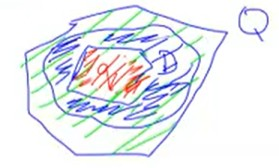
\includegraphics{curveD.jpg}

\Def
{
Нижней площадью $\underline{S}(D) = \sup S(q)$ называем максимальный по площади подмногоугольник множества $D$, Верхней площадью $\overline{S}(D) = \inf (S(Q))$  назовем минимальный описанный многоугольный вокруг $D$. Если $\underline{S}(D) = \overline{S}(D) $, то будем говорить что $D$ квадрируема и $S(D) = \overline{S}(D) = \underline{S}(D)$
}

\textbf{Свойства:}
\begin{enumerate}[1)]
	\item $D = D'\cup D'', D'\cap D'' = \varnothing \Rightarrow S(D) = S(D') + S(D'')$
	\item $D'\subset D$ $\Rightarrow$ $S(D') \leq S(D'')$
	\item $S(D) \geq 0$
\end{enumerate}

Заметим что площадь криволинейной трапеции - площадь под графиком функции, где верхние и нижние суммы Дарбу соответствуют верхним и нижним площадям, так же очевидно является аддитивной функцией промежутка

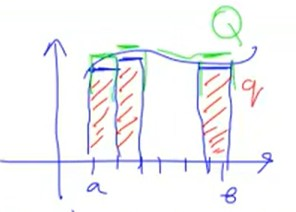
\includegraphics{сurvefunc.jpg}

\Def
{ \[
	\begin{cases}
		\int\limits_a^b f(x)dx - \text{Алгебраическая площадь} \\
		\int\limits_a^b |f(x)|dx - \text{Собственная площадь}
	\end{cases}
	\]
}
\item \textbf{Объем тела вращения} 

\Def
{
Определим $V(D)$ аналогично площади $S(D)$ - совпадение описанных и вписанных объемов многогранников, проводим аналогичные рассуждения про объем тела вращения графика функции вокруг оси
}

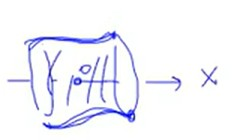
\includegraphics{сurveV.jpg}

\formula{\label{eq:funcV}
 (b-a) \pi (\inf\limits_{x\in[a, b]} f(x))^2\leq V(a ,b) \leq \pi (\sup\limits_{x\in[a, b]} f(x))^2(b-a) \Rightarrow V(a, b) = \int\limits_a^b \pi f^2(x)dx
}

\item \textbf{ Плошадь криволинейного сектора}

\[
f: [a, b] \to \R,  \ \ f\in C[a ,b] :
\begin{cases}
	x = r\cos(\phi) \\
	y = r\sin(\phi)
\end{cases}
 y = f(x) \Leftrightarrow r = r(\phi)
\]3

\begin{multicols}{2}
	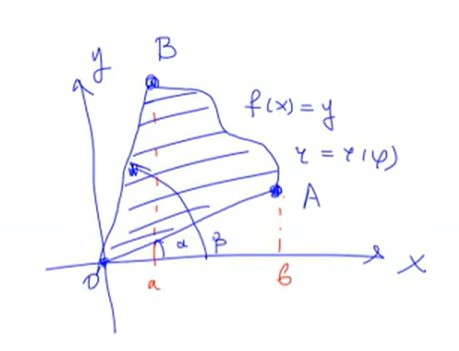
\includegraphics[scale = 0.7]{curvepolar.jpg}
	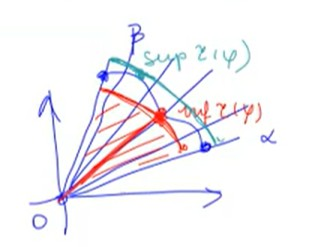
\includegraphics{curvepolar2.jpg}
\end{multicols}

Аналогично рассматриваем максимальный вписанный и минимальный описанный сектора, где площадь сектора $S = r^2 \phi/2$

\formula
{
S = \dfrac{1}{2}\int\limits_{\phi_1}^{\phi_2} r^2(\phi) d\phi
}
\end{enumerate}

\subsection{Гиперболические функции}

Будет скоро (наверное, когда оптимизирую производство своих рисунков)

\section{Несобственные интегралы}

\subsection{Несобственные интегралы первого рода}

\Def
{\label{def:notmyint}
\[
f: [a, +\infty) \to \R, \ \  \forall b > a f\in \Re[a, b] 
\]	
Несобственным интегралом первого рода называется
\[
\int\limits_a^{+\infty} f(x)dx = \lim\limits_{b \to +\infty} \int\limits_a^b f(x)dx = \lim\limits_{b \to +\infty} F(x)
\]

В том случае, если такой предел существует и конечный, интеграл называется сходящимся. Заметим, что в таком случае "хвост" интеграла должен стремиться к  нулю:
\[
\lim\limits_{b \to +\infty} \int\limits_b^{+\infty} f(x)dx = 0
\]

Если предел несобственного интеграла первого рода не существует или бесконечен, то интеграл называют расходящимся.

Если $f: (- \infty, a] \to \R$, то интеграл определяется аналогично

Для существования интеграла с бесконечными пределами необходимо, чтобы функция была интегрируема на всем множестве $\R$ существовали небесконечные  оба выше описанных предела:
\[
\int\limits_{-\infty}^{+\infty} f(x)dx = \int\limits_{-\infty}^{a} f(x)dx +  \int\limits_a^{+\infty} f(x)dx 
\]
}

\Def
{ \label{def:intmain}
Интегралом в смысле главного значения (интегралом в случае Коши) называется:
\[
v.p. \ \int\limits_{-\infty}^{+\infty} f(x)dx = \lim\limits_{b \to +\infty} \int\limits_{-b}^b f(x)dx
\]

Замечание:
\[
\exists \in \R  \ \ \int\limits_{-\infty}^{+\infty} f(x)dx  \Rightarrow \exists v.p. \int\limits_{-\infty}^{+\infty} f(x)dx  = \int\limits_{-\infty}^{+\infty} f(x)dx
\]
\[
\nexists \in \R v.p. \int\limits_{-\infty}^{+\infty} f(x)dx \Rightarrow \nexists \int\limits_{-\infty}^{+\infty} f(x)dx
\]
}

\paragraph{Простейшие свойства и условия сходимости несобственных интегралов}

\begin{enumerate}
	\item 
	\[
	\int\limits_a^{+\infty}f(x)dx
	\]
\end{enumerate}





\

\lecture

\


\

\lecture

\part{Ряды}

\section{Основные числовые понятия}

\subsection{Определения}

\Def{ \label{def:sum}
$\sum\limits_{n = 1} ^{\infty} a_n, \ a_n \in \R ( \im)$, $a_n$ - общий член ряда 

$\Sum a_n$ - частичная сумма ряда, $r_n = \sum\limits_{k = n + 1} ^{\infty} a_n $ - остаток ряда 

$\Sum a_n = S_n$, Если $\exists \lim_{n \ri \infty} S_n$, то ряд называют сходящимся, если $\nexists$ или $\infty$ - расходящимся
}

 \noindent \ex $ \SUM q^n$
При q < 1
\formula{
S_n = \Sum q^k  = \dfrac{1- q^{n+1}}{1-q} 
}
\[ \exists \lim_{n\ ri \infty} = \dfrac{1}{1-q} = S\]
При q > 1 расходится

 \noindent \textbf{Необходимое условие сходимости}: 
\[\Lim a_n = 0 \Leftrightarrow a_n = S_n - S_{n-1} \to 0\]

 \noindent \textit{Но не достаточное условие}

 \noindent\ex Гармонический ряд
 \[\SUM \dfrac{1}{n}, \ \ \ 0 < \ln(1+\dfrac{1}{n}) < \dfrac{1}{n}\]
 \[\Sum \ln(k+1) - \ln(k) = \ln(n+1) < \Sum \dfrac{1}{n}\] 
 
 \subsection{Простейшие свойства и условия сходимости числовых рядов}
 
\begin{enumerate}
	\item $\SUM a_n \ \ \SUM b_n $ - сходящиеся ряды
	
	 $\forall \lambda \in \R (\im ) \Rightarrow \SUM (a_n + \lambda b_n)$  - так же сходятся
	
	 $a_n, b_n$ - расходятся $\Rightarrow \fbox{?}$
	
	\ex $\SUM (\pm 1 +q^n)$
	
	 $\SUM a_n$ - расходится $\Rightarrow$ $\SUM \lambda a_n$ - расходится
	\[\Let \SUM (a_n + b_n) - \text{ пусть сходится, разобьем на пару:}\]
	\[\SUM(a_n + b_n + (-b_n))\]
	\item Сгруппированные ряды $\SUM A_k$
	 \[\SUM a_n = a_1 + a_2 + \cdots \Rightarrow \underline{a_1 + a_2 + a_3 \cdots a_m}_{A_1}  + a_{m + 1} \cdots \]

\textbf{\underline{Утверждение 1}}
\formula{
\SUM a_n \text{    сх} \Rightarrow \SUM A_k \text{  сх}
}
\textbf{\underline{Доказательство}}
\[\sigma_m = \SuM A_k = a_1 + a_2 \cdots + a_{n_{m}} = S_{n_{m}} \to S = \Lim a_n \]

\fbox{Обратное верно не всегда }

\ex $\SUM (-1)^n$

\ubf{Утверждение}
\formula{\SUM A_n \text{  сх}, \forall k \ \forall n',n'' \ \ \  a_{n'} \cdot a_{n''} \geq 0 \Rightarrow \SUM a_n \text{\textit{сходится к тому же пределу}}}
То есть слагаемые одного знака

 \ubf{Доказательство:}

\[\sigma_m = \SuM A_k \to \sigma \ \ \exists\]
\[S_n = \Sum a_n = \sigma_{m_0} + a_{nm{_0}} + \cdots \Text{неполное $A_{m_0+1}$}\]
\[S_n = \sigma_{m_0} + \underline{O}(A_{m_0+1}) \to \sigma\]
 
\ubf{Утверждение}

\formula{\SUM A_n - \Text{сх}, \Lim a_n = 0 \Rightarrow \exists C > 0: \forall k |\{a_{n_k}\}| < C, \Rightarrow \SUM a_n\Text{сх}}

\ubf{Доказательство:}

Выносим $\sup a_{n_m}$ в остатке суммы: $S_n = \sigma_{m_0} + a_{n_m} \cdots \leq \sigma_{m_0} + C \sup a_{m_0} \to \sigma $
\item \[\SUM a_n \Text{сх} \ \  \forall m = const \Leftrightarrow  r_m =  \sum\limits_{k = m + 1}^{\infty} a_n \  \Text{сх}\]

\ubf{Доказательство}
\[S_n = \Sum a_k = S_m + r_m \to S_m + r_m \Rightarrow r_m = S - S_m = const \]
\underline{Замечание:} это свойство позволяет при изучении сходимости ряда выбрасывать из него конечное число слагаемых, что не скажется на сходимости ряда

\ubf{Следствие} \[\SUM a_n \Text{ сх} \Leftrightarrow r_m \to 0, m \to \infty\]
\[n \to \infty \Rightarrow S - S_m = r_m \Rightarrow r_m = 0\]
Обратное доказывается аналогично

\item \ubf{Критерий Коши} 
\formula{\SUM a_n \Text{  сх} \Leftrightarrow \exists \in \R \Lim S_n \Leftrightarrow\ \foralle \exists N \ \ \forall n > N \ \forall p > 0 |S_{n+p} - S_n| < \epsilon}

\ex $\SUM \dfrac{1}{n^2}$
\[\dfrac{1}{k^2} <\dfrac{1}{k(k-1) } = \dfrac{1}{k-1} - \dfrac{1}{k} \Rightarrow \Sum \dfrac{1}{k^2} < \dfrac{1}{k} \]

\item \[\SUM|a_n| \Text{  сх} \Rightarrow \SUM a_n \Text{  сх}\]

\ubf{Доказательство} 

Записать критерий Коши

\section{Знакопостоянные ряды}

Знакопостоянными рядами считаем те, которые стабилизируются начиная с какого то момента

\subsection{Интегральный признак}
\[a_n \geq 0 \ \ \forall n \in \N \]

\Theorem{Критерий сходимости знакопостоянного ряда}{\label{Th:endsum}$\SUM a_n$- сходится $\Leftrightarrow$ $\SUM a_n$ - ограничена сверху}{ Функция монотонная возрастает и ограничена сверху, следовательно существует конечный предел $S_n$}

\Theorem{Интегральный признак Коши}{\label{Th:intsignKoshi} \[ f : [0, +\infty ] \to [1, +\infty] \ \ \forall n \ f(n) = a_n \Rightarrow \exists \SUM a_n \Leftrightarrow \int\limits_{1}^{\infty} f(x)dx \]}{
\[f \Text{неубывающая } \Rightarrow \forall b > 1 \ \ f \in \Re[a, b]\]

\[a_{n+1} = f(n+1) \leq \int\limits_n^{n+1} f(x)dx \leq f(n) = a_n\]
\[\Sum a_{k+1}  \leq \int_1^{\infty} f(x)dx \leq \Sum a_k\]
Далее если сходится ряд, то интеграл ограничен, соответственно сходится

Если сходится интеграл, то $S_n+1$ ограничена сверху $\Rightarrow$ сходится по свойствам рядам

\textit{Геометрическая интерпретация - функция и верхняя сумма Дарбу $\Rightarrow$  Верхние треугольники составляют не более чем $a_1$ }
}
\end{enumerate}
\ex \[\SUM \dfrac{1}{n^p}, \begin{cases}
	p>1 \Text{ Сходится } \\
	p \leq 1 \Text{ Расходится}
\end{cases}\]
Таким образом можно (заменой переменной, например) поджимать ряды интегралом
\subsection{Признаки сравнения}
\Theorem{Первый признак сравнения}{\label{Th:firstsignsums}
	\[\SUM a_n, \SUM b)n, \forall n \ \ 0 \leq a_n \leq b_n\]}{
\begin{enumerate}
	\item $b_n$ сходится $\Rightarrow$ $a_n$ ограничено, cходится
	\item $a_n$ расходится $\Rightarrow b_n$ расходится - неограничено
	\item $\exists \Lim \dfrac{a_n}{b_n} \Rightarrow$ сходимость одинаковая
\end{enumerate}
}

\ubf{Второй признак сравнения} :
\[
a_n \sim k \cdot \dfrac{1}{n^p} \Leftrightarrow \Text{  \ \ \  Сходимости аналогчины}
\]

\ubf{Третий признак сравнения}
\[
\dfrac{a_{n+1}}{a_n} \leq \dfrac{b_{n+1}}{b_n}, \ \ a_n, b_n > 0
\]
\begin{enumerate}
	\item 
	\[
	 \SUM b_n \Text{ сх} \Rightarrow \SUM a_n \Text{  cx}
	\]
	\item 
	\[
	\SUM a_n \Text{ расх} \Rightarrow \SUM b_n \Text{ расх}
	\]
\end{enumerate}
\subsection{Признаки Даламбера и Коши}

\Theorem{Признак Даламбера}{\label{Th:signD'alamber}
Если $\exists \ \Lim \dfrac{a_{n+1}}{a_n} = a$
\begin{enumerate}
	\item $d < 1 \ \Rightarrow \SUM a_n$ сходится 
	\item $d > 1 \ \Rightarrow \SUM a_n$ расходится
\end{enumerate}
}{
\[ 
\Let d = \Lim \dfrac{a_{n+1}}{a_n} < , \ \ \exists \forall N  \ \forall n > N \ \ \dfrac{a_{n+1}}{a_n} \leq q < 1
\]
\[
\dfrac{a_{n+1}}{a_n} < \dfrac{q^{n+1}}{q_n} \Rightarrow \Text{ По третьему признаку сравнения сходится} 
\]
\fbox{Важно: q < 1}
Обратное доказывается аналогично
}

\Theorem{
Признак Коши
}
{\label{Th:signKoshi}
Если $\exists \Lim \sqrt[n]{a_n} = k$:
\begin{enumerate}
	\item $k < 1  \Rightarrow \SUM a_n$ сх 
	\item $k > 1 \Rightarrow \SUM a_n $ расх
	\item $k = 1 \Rightarrow$ \fbox{?}
\end{enumerate}
}{
Основывается на третьем признаке сравнения:
\[
k = \Lim \sqrt[n]{a_n} < 1 \Rightarrow \exists \ \forall n > N \ \ \sqrt[n]{a_n} \leq q < 1 \Rightarrow a_n \leq q^n
\]
Но $\SUM q^n $ сходится $\Rightarrow$ по первому признаку сходимости 
Обратное доказывается аналогично
}

\ubf{Непредельная форма Даламбера Коши} 

Аналогичны, но без пределов
\newpage
\lecture

\subsection{Признаки Куммера, Раабе, Бертрана, Гаусса}




\Theorem{Признак Куммера}{\label{Th:signKummer}
	\[ \forall n \ \{ c_n \}^{\infty}, c_n > 0 \]
	\[\Text{Если } \exists N \ \ \forall n  \ \ \ \kappa_n =  c_n \dfrac{a_n}{a_{n+1}} - c_{n-1}\]
	
	\begin{enumerate}
		\item 
		$ \kappa_n \geq q >0 \Rightarrow \SUM a_n \Text{ сх} $
		\item 
		$\kappa_n \leq 0$ и $\SUM \dfrac{1}{c_n}$ расх 
		$\Rightarrow \SUM a_n \Rightarrow$ расх
	\end{enumerate}
}{
	\[N = 1, \ \forall  n \geq N \ \ \Let \kappa_n \geq q > 0\]
	
	\[c_na_n - c_{n+1}a_{n+1} \geq q a_{n+1} >0 \]
	\[(c_na_n)^{\infty} \Text{монотонно убывает, положителен $\Rightarrow$ Существует конечный пределе $ c_na_n$ } \]
	\[c_na_n - c_{n+1}a_{n+1} \geq q a_{n+1} >0 \Rightarrow \Text{Поджат сверху $ca_n$ по первому признаку сходится} \]
	\formula{ \SUM \dfrac{1}{c_n} \Text{  расх  } \kappa_n \leq 0 \Rightarrow \dfrac{a_{n+1}}{a_n} \geq \dfrac{1/c_{n+1}}{1/c_n} }
	
	По третьему признаку сходится}



\ubf{Предельная форма}

Если существует и конечный $\Lim \kappa_n = \kappa$, то
\begin{enumerate}
\item $\kappa$ >0 $\Rightarrow$ $\SUM a_n$ сходится
\item $\kappa$ < 0 $\Rightarrow$ $\SUM a_n $расх
\end{enumerate}

\textit{Cледствия}

\[c_n = 1 \Rightarrow \SUM \dfrac{1}{c_n} \Text{расх} \ \ \kappa_n \dfrac{a_n}{a_{n+1} - 1} \Rightarrow \dfrac{1}{a} -1 > 0 \Text{   сх, иначе расходится}
\]
Гармонический ряд
\[
c_n = n \Rightarrow \SUM \dfrac{1}{n} \Text{расходится} 
\]
\[
\kappa_n = n \dfrac{a_n}{a_{n+1}} - (n+1) = n ( \dfrac{a_n}{a_{n+1}} - 1) - 1
\]
\ubf{Признак Раабе (предельная форма):} \label{Th:signRaabe}

Если существует и конечный $\Lim n(\dfrac{a_n}{a_{n+1}}-1) > 1 \Rightarrow \SUM a_n$  сходится, иначе расходится ($n(\dfrac{a_n}{a_{n+1}}-1) = \rho_n$)

\fbox{Признак Раабе сильнее Даламбера(определенность при единице)}

\ubf{Признак Бертрама} \label{Th:signBertram}

Если существует конечный предел \[\Lim \beta_n = \Lim \ln n \rho_n  = \beta \Rightarrow \begin{cases}
\beta > 1 \Rightarrow \SUM a_n \Text{сходится} \\ 
\beta < 1 \Rightarrow \SUM a_n \Text{расходится}
\end{cases}
\]

\ubf{Признак Гаусса} \label{Th:signGauss}

\[\exists N \ \forall n > N\]
\[\dfrac{a_n}{a_{n+1}} = \lambda + \dfrac{\mu }{n} + \dfrac{\theta_n}{n^{1+\epsilon}}, \ \ \theta_n \Text{огранчиена}\]
\begin{enumerate}
\item \formula{\lambda > 1 \Rightarrow \Sum a_n  \Text{   cх}}
\item \formula{ \lambda < 1 \Rightarrow \Sum a_n  \Text{  раcх}}
\item \formula{\lambda = 1 \Rightarrow 
\begin{cases}
	\mu > 1 \Rightarrow \SUM a_n \Text{  cx} \\ 
	\mu < 1 \Rightarrow \SUM a_n \Text{  pacx}
\end{cases}}
\end{enumerate}
\ubf{Доказательство} 

1, 3 $\Rightarrow$ очевидно по признаку Даламбера (см. стр. \pageref{Th:signD'alamber})

2 $\Rightarrow \rho_n = \mu + \dfrac{\theta_n}{n^{\epsilon}} \Rightarrow $ признак Раабе (см стр. \pageref{Th:signRaabe})

\[\beta_n = \ln n(\rho_n -1) = \ln n \dfrac{\theta_n}{n^\epsilon} \Rightarrow \beta < 1 \Text{ряд расходится}\]

\section{Знакопеременные ряды}

Нельзя найти такое $N$, чтобы $\forall n > N \ \ a_n $ имеет один и тот же знак

\Def{\label{def:ifsum} $\SUM a_n$ называется условно сходящимся если $\SUM a_n$ сходится, но $\SUM |a_n|$ - расходится}

\[\SUM a_n \ \ a(t) = a_n \ \ t \in [n, n+1] \ \ \forall x \ \in \R \ \exists n \in \N: \ x \in [n, n+1)\]

Покажем, что сходимость ряда равносильна сходимости кусочно непрерывного $\int\limits_{1}^{\infty} a(t)dt$

\ubf{Утв} :\[ \SUM a_n \Leftrightarrow \int\limits_{1}^{\infty} a(t)dt \]

\ubf{Доказательство}

\[(\Rightarrow) \ \exists \Lim S_n = \Sum a_k\]
\[\int\limits_{1}^{x} a(t)dt = S_{n-1}  + a_n(x-n), \ \  0 \leq (x - n) \leq 1 \to a_n(x-n) \to 0 \Rightarrow \ \exists \int\limits_{1}^{\infty} a(t)dt = S\]
\[(\Leftarrow) \ \ \exists \int\limits_{1}^{\infty} a(t)dt \Leftrightarrow \foralle \exists A > 1 \forall \ \ x'x'' > A \ \ | \int\limits_{x'}^{x''} a(t) dt| < \epsilon\]

\[\Let x'= n, \ \ x" = n + p \ \ \forall p > 0, N = [A]\]
\[\int\limits_{n}^{n+p} a(t)dt = |S_{n+p} - S-n| = |\sum\limits_{k = n}^{n+p-1} a_k| < \epsilon \Rightarrow \Text{По критерию Коши}\]

\ubf{Признак Дирихле}\label{Th:signDirihle}
\[\sphericalangle \SUM a_nb_n\] 
\[
\begin{cases}
	 \ \ \exists C \ \ \forall N  \ \ |\Sum a_k| \leq C\\
b_n \Text{монотонно убыывает} \\
b_n \to 0
 \end{cases}
\]
\ubf{Доказательство}

\[a_n \to a(t), \ \ b_n \to b(t), \ \ A_n = \Sum a_k\]
\[\SUM a_nb_n \Leftrightarrow \int\limits_{1}^{\infty} a|t|b|t|dt\]
\[\left|\int\limits_{1}^{x} a(t)dt\right| = |A_{n-1} + a_n(x-n)| \leq |A_{n-1}| + |a_n| \leq C + 2C = 3C (|a_n| = |S_{n} - S_{n-1}| \leq 2C)\]
\[\Rightarrow \ \forall x \ \ \left|\int\limits_{1}^{x} a(t)dt\right| \leq 3C\]
Но $b_n$  бежит к нулю, значит по признаку Дирихле $\int\limits_{1}^{\infty} a(t)b(t)dt$ сходится

\subsection{Знакочередующиеся ряды. Признак Лейбница}

\Def{\label{def:sumsignchange}
\[
\SUM (-1)^{n+1} b_n, b_n \geq 0 \ \ \forall n
\]
Называется знакочередующимся рядом (Рядом Лейбница)
}

\Theorem{Признак Лейбница}{\label{Th:signLeibnitc}Если $b_n \to 0$, то знакочередующийся ряд сходится }{
\[
\begin{cases}
	a_n = (-1)^{n+1} \\ b_n = b_n
\end{cases}
\Rightarrow Принцип Дирихле
\]
\ex
\[\SUM (-1)^{n+1} \dfrac{2+(-1)^n}{n} \Text{  \ \ Ряд Лейбница  }\]
Монотонность отсутствует $\Rightarrow$ признак Лейбница \textbf{не работает}
}

\Theorem{Теорема об остатке знакочередующегося ряда}{\label{Th:signremainder}
$\SUM (-1)^{n+1} b_n$ сходится $\Rightarrow \ \ r_m = \sum\limits_{k = m + 1}^{\infty} (-1)^{k+1} b_k = (-1)^{m+1} b_{m+1} \theta, \ \ 0 \leq \theta \leq 1 $
}{
Покажем, что сумма ряда не превосходит первого члена и положительна:
\[
b_1 - b_2 + b_3 - \cdots + b_{2k+1} - b_{2k+2} + \cdots
\]
Заметим, что все сгруппированные ряды сходятся и  $b_n \to 0$ монотонно $\Rightarrow$ попарно сгруппируем $b_n$ 
\[
\Sum A_k = \Sum b_{2k+1} - b_{2k+2}, \ \ A_k \geq 0 \Rightarrow \Sum A_k \geq 0 \Rightarrow A_k \to S
\]
Теперь сгруппируем со сдвигом на 1 элемент
\[
\Sum A_k  =  \Sum  - b_{2k} - b_{2k+1} \ \leq A_0 \Rightarrow \Sum A_k \to S \Rightarrow 0 \leq S \leq b_1,
\]
Рассмотрим $r_m$ как последнюю сумму $\Rightarrow 0 \leq r_m < b_{m+1} \Rightarrow r_m = \theta b_{m+1}, \ \ \theta \in [0, 1]$
}

\end{document}